\documentclass[12pt]{article}
\usepackage[utf8]{inputenc}
\usepackage[margin=1in]{geometry}
\usepackage{xcolor}
\usepackage{listings}
\usepackage{dirtree}
\usepackage{nameref}
\usepackage{amsfonts}
\usepackage{tikz}
\usetikzlibrary{positioning}
\usepackage{float}
\usepackage{hyperref}
 
\usepackage{color}   %May be necessary if you want to color links
\usepackage{hyperref}
\hypersetup{
    linktoc=all,     %set to all if you want both sections and subsections linked
}
\usepackage[utf8]{inputenc}
\usepackage{menukeys}

\definecolor{mGreen}{rgb}{0,0.6,0}
\definecolor{mBlue}{rgb}{0,0,1}
\definecolor{mRed}{rgb}{0.64, 0.08, 0.08}
\definecolor{backgroundColour}{rgb}{0.95,0.95,0.92}

\lstdefinestyle{CStyle}{
    backgroundcolor=\color{backgroundColour},   
    commentstyle=\color{mGreen},
    keywordstyle=\color{mBlue},
    numberstyle=\tiny\color{mBlue},
    stringstyle=\color{mRed},
    basicstyle=\footnotesize,
    breakatwhitespace=false,         
    breaklines=true,                 
    captionpos=b,                    
    keepspaces=true,                 
    numbers=left,                    
    numbersep=5pt,                  
    showspaces=false,                
    showstringspaces=false,
    showtabs=false,                  
    tabsize=4,
    extendedchars=true,
    literate={à}{{\'a}}1 {è}{{\`e}}1 {é}{{\'e}}1 {î}{{\^i}}1,
    language=C
}

\lstdefinestyle{BashStyle}{
    backgroundcolor=\color{backgroundColour},   
    commentstyle=\color{mGreen},
    keywordstyle=\color{mBlue},
    numberstyle=\tiny\color{mBlue},
    stringstyle=\color{mRed},
    basicstyle=\footnotesize,
    breakatwhitespace=false,         
    breaklines=true,                 
    captionpos=b,                    
    keepspaces=true,                 
    numbers=left,                    
    numbersep=5pt,                  
    showspaces=false,                
    showstringspaces=false,
    showtabs=false,                  
    tabsize=4,
    extendedchars=true,
    literate={à}{{\'a}}1 {è}{{\`e}}1 {é}{{\'e}}1 {î}{{\^i}}1,
    language=Bash
}

\title{Manuel d'utilisation Projet JAVA : Partage de butin}
\author{EL MONTASER Osmane TD1 et VIDART Paul TD1}
\date{}

\begin{document}

\begin{titlepage}
\maketitle
\end{titlepage}

\renewcommand*\contentsname{Sommaire}
\tableofcontents
\pagebreak

\section{Instructions pour utiliser notre programme}
\subsection{Création d'un équipage de pirates}


\subsubsection{Ajout des pirates}
\paragraph{} Pour ajouter les pirates à l'équipage, il suffit de renseigner le nombre de pirates au lancement du programme en répondant à la première question :
\begin{figure}[H]
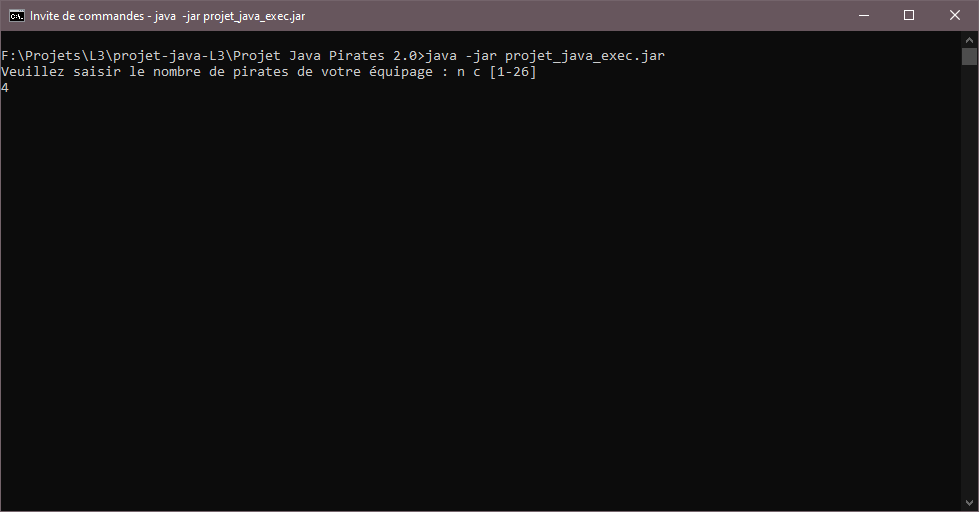
\includegraphics[width=16cm]{ajout_pirate}
\centering
\caption{Création d'un équipage de 4 pirates}
\end{figure}
Pour l'instant, chaque pirate se voit affecter automatiquement d'un nom provenant d'une lettre de l'alphabet [A-Z]. Ce qui rend impossible la création d'un équipage de plus de 26 pirates. Si vous avez tout bien fait, le terminal devrait afficher ceci :
\begin{figure}[H]
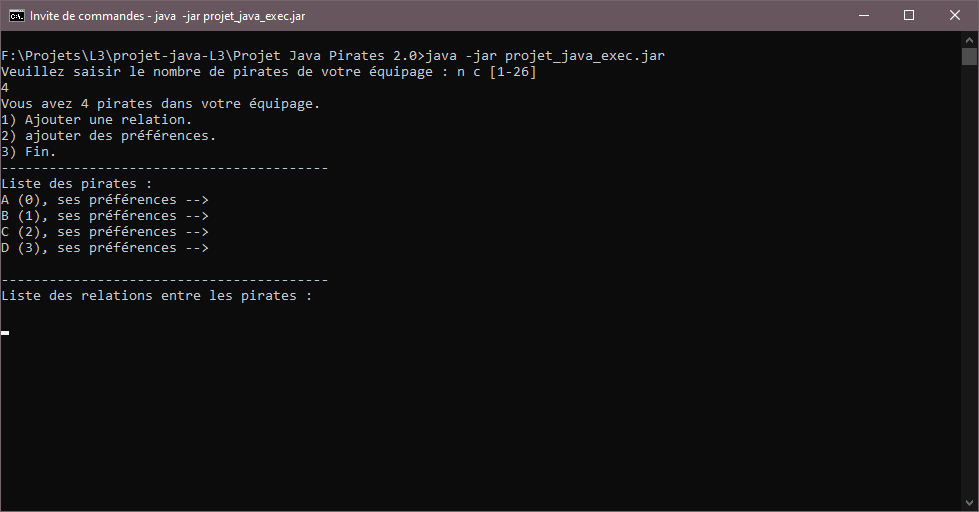
\includegraphics[width=16cm]{main_menu}
\centering
\caption{Équipage de 4 pirates généré et affiché}
\end{figure}
\textbf{Vous ne pourrez pas passer à la résolution du problème tant que vous n'avez pas donné les préférences de chaque pirate.}
\begin{figure}[H]
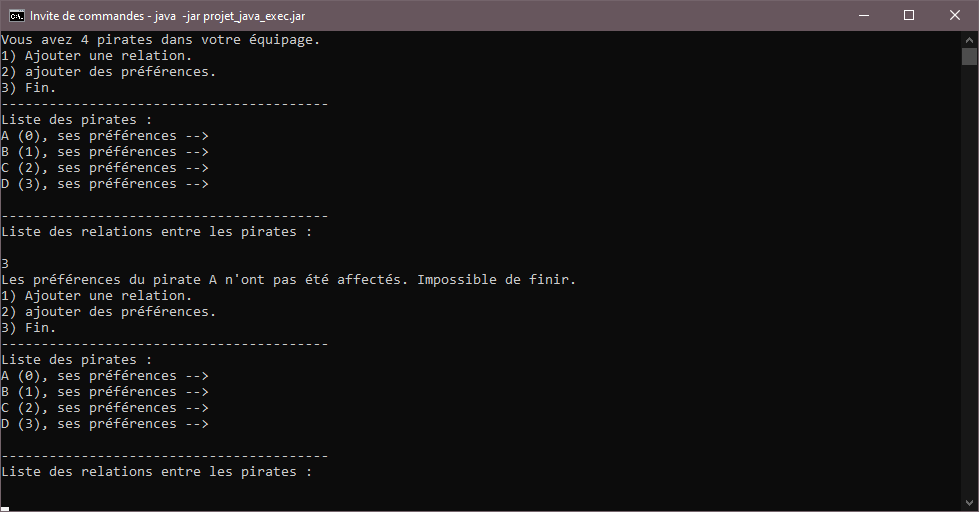
\includegraphics[width=16cm]{erreur_pref}
\centering
\caption{Impossible de terminer sans donner toutes les préférences}
\end{figure}


\subsubsection{Ajout des relations entre pirates}
\paragraph{} Pour ajouter une relation entre 2 pirates, il suffit de taper 1 dans le menu suivant :
\begin{figure}[H]
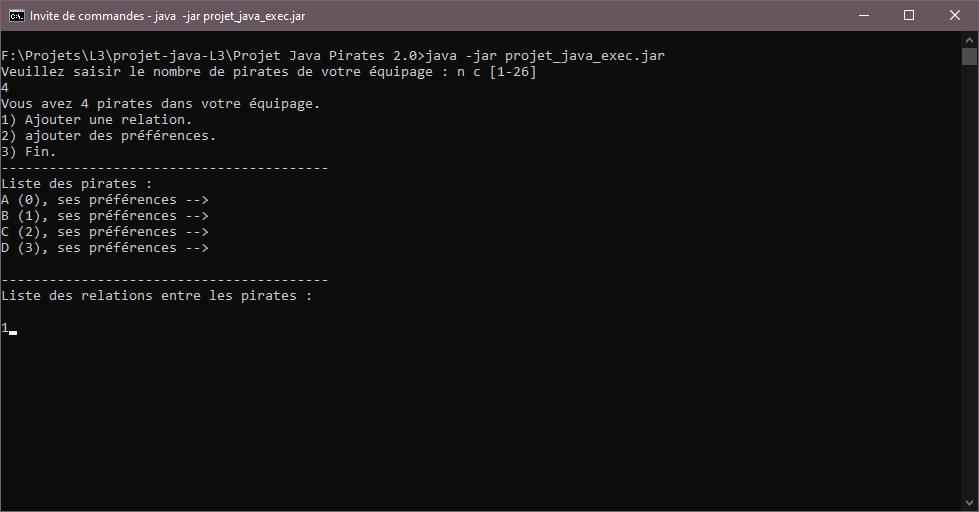
\includegraphics[width=16cm]{ajout_relation_1}
\centering
\caption{Sélection de l'option 1, "Ajout d'une relation"}
\end{figure}
Puis tapez la lettre correspondante aux 2 pirates, ici le pirate A n'aime pas le pirate B (et vice-versa) :
\begin{figure}[H]
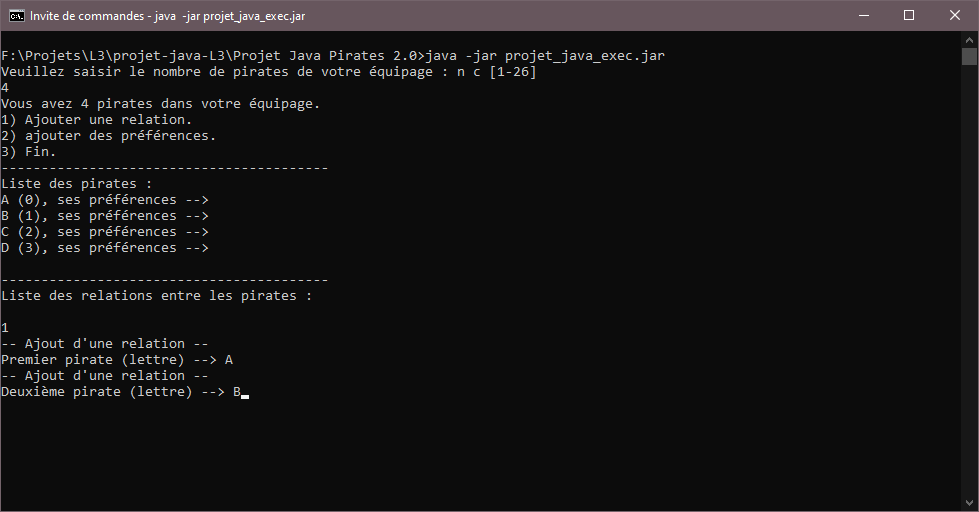
\includegraphics[width=16cm]{ajout_relation_2}
\centering
\caption{Ajout de la relation Pirate A n'aime pas Pirate B}
\end{figure}

Appuyez sur \keys{Enter} et vous retournerez au menu principal, où vous pourrez voir le résultat de l'opération :
\begin{figure}[H]
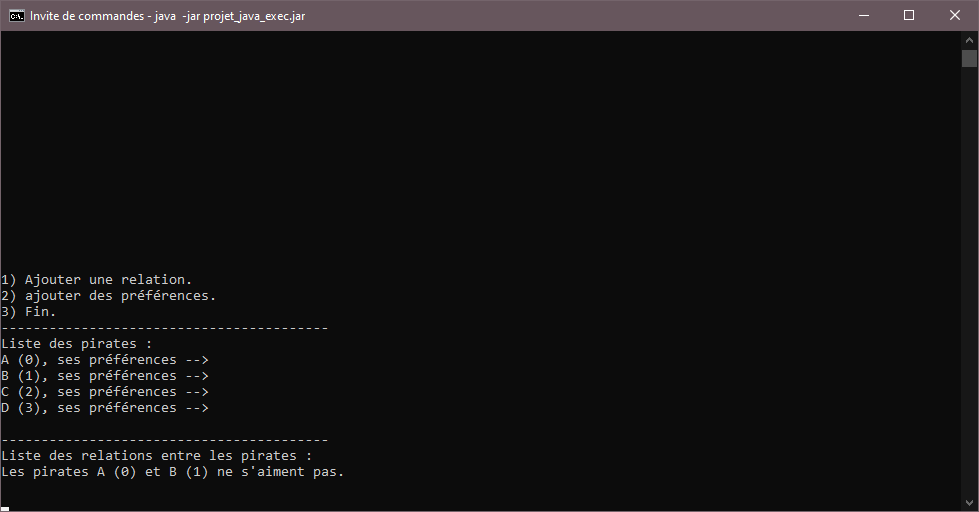
\includegraphics[width=16cm]{ajout_relation_3}
\centering
\caption{Résultat : Ajout de la relation Pirate A n'aime pas Pirate B}
\end{figure}


\subsubsection{Ajout des préférences des pirates}
\paragraph{} Pour pouvoir calculer le coût d'une solution, il faut d'abord renseigner les préférences de chaque pirate. Vous devez taper 2 sur le menu suivant :
\begin{figure}[H]
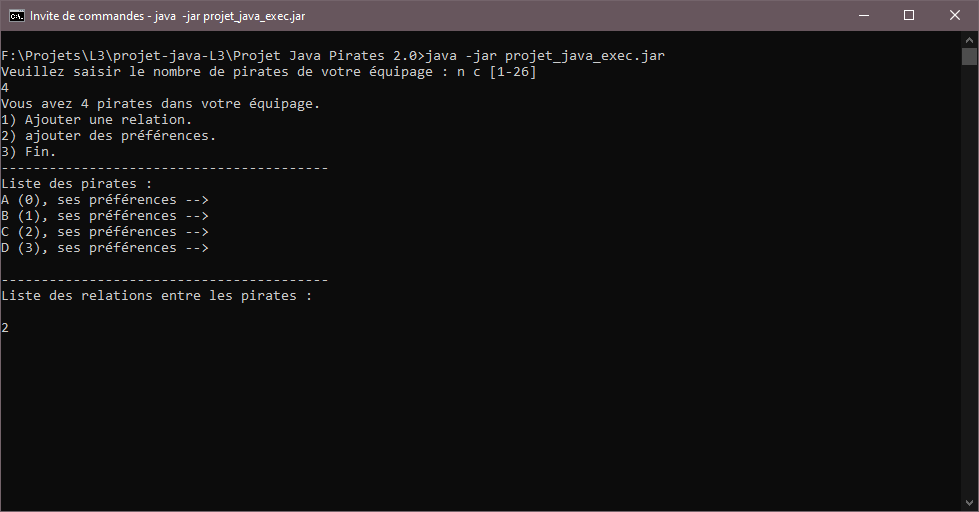
\includegraphics[width=16cm]{ajout_pref_1}
\centering
\caption{Sélection de l'option 2, "Ajout des préférences"}
\end{figure}
Il vous sera alors demander de taper \textbf{en une ligne} séparé par \textbf{un espace}, la lettre du pirate, le numéro de chaque trésor ranger dans l'ordre décroissant de ses préférences. Voici un exemple pour le pirate A avec les préférences $o1>o2>o3>o4$ :
\begin{figure}[H]
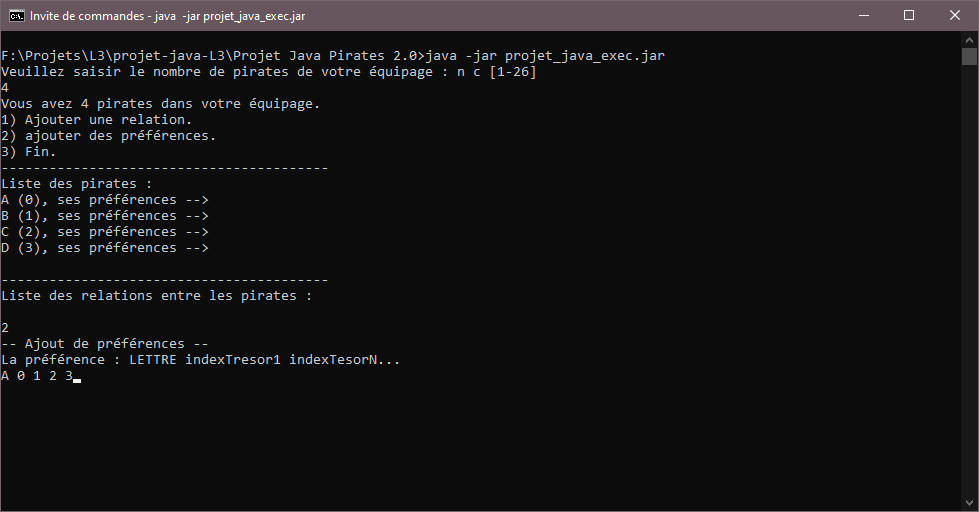
\includegraphics[width=16cm]{ajout_pref_2}
\centering
\caption{Ajout des préférences $o1>o2>o3>o4$ sur le pirate A}
\end{figure}
Appuyez sur \keys{Enter} et vous retournerez au menu principal, où vous pourrez voir le résultat de l'opération :
\begin{figure}[H]
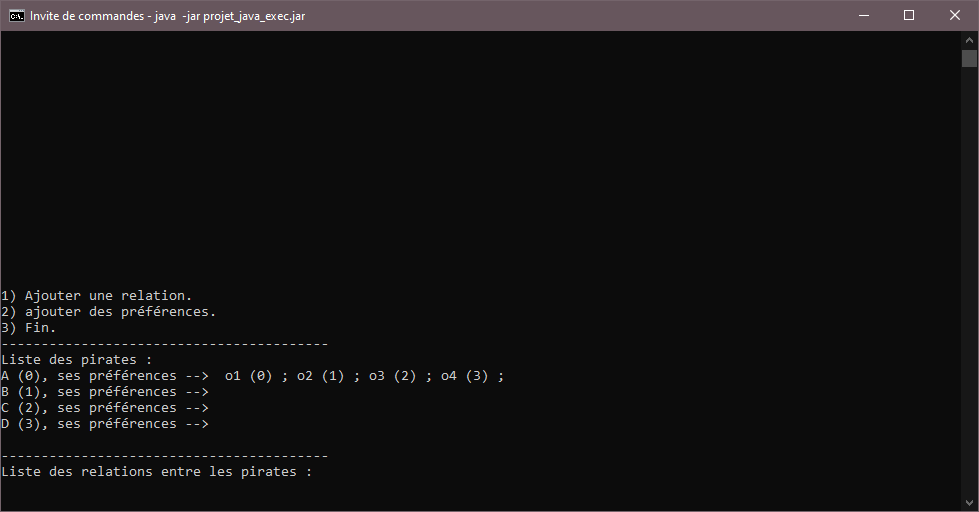
\includegraphics[width=16cm]{ajout_pref_3}
\centering
\caption{Résultat : Ajout des préférences $o1>o2>o3>o4$ sur le pirate A}
\end{figure}

\subsection{Génération d'une solution}
\paragraph{} Une fois que vous avez ajouté toutes les relations entre les pirates et les préférences de chaque pirate, vous pourrez taper 3 dans le menu de création d'équipage. Le terminal devrait alors afficher ceci :
\begin{figure}[H]
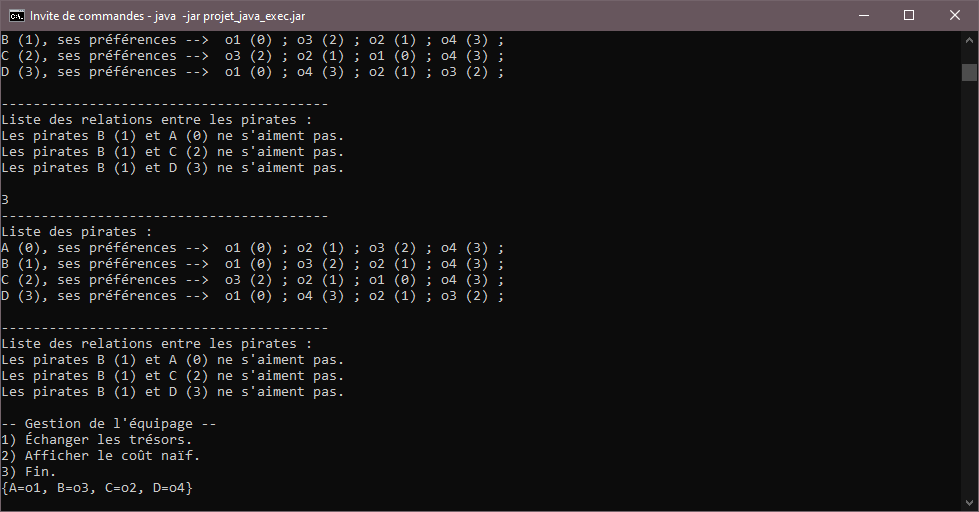
\includegraphics[width=16cm]{menu_gestion}
\centering
\caption{Menu de gestion du butin}
\end{figure}
Vous pourrez alors voir toutes les informations sur votre équipage ainsi qu'une attribution naïve automatiquement proposée à la fin.

\subsubsection{Échanger le butin entre 2 pirates}
Vous pouvez échanger le butin entre les pirates en tapant 1 puis les lettres des 2 pirates entre qui échanger le butin :
\begin{figure}[H]
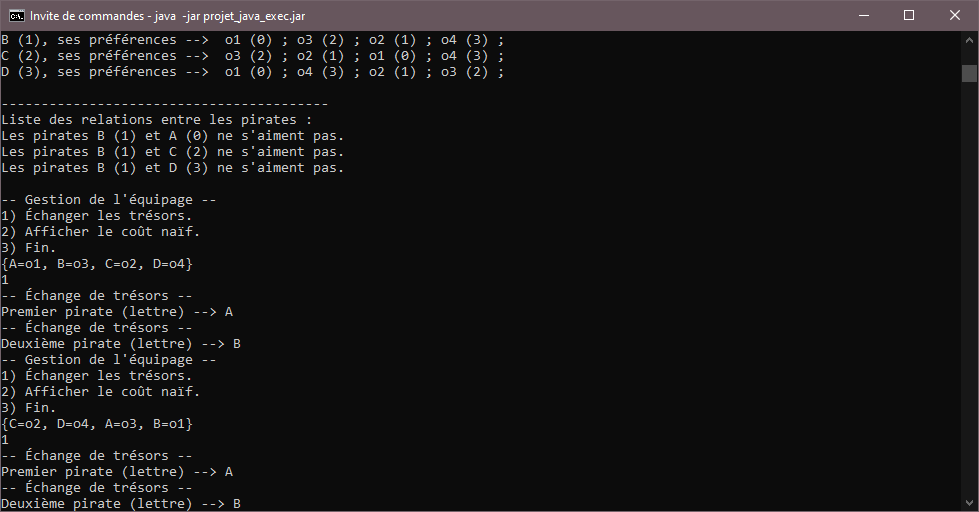
\includegraphics[width=16cm]{swap}
\centering
\caption{Échange des trésors entre le pirate A et le pirate B}
\end{figure}
\subsubsection{Calcul du coup naïf}
Pour afficher le coût de la solution naïve, il suffit de taper 2 :
\begin{figure}[H]
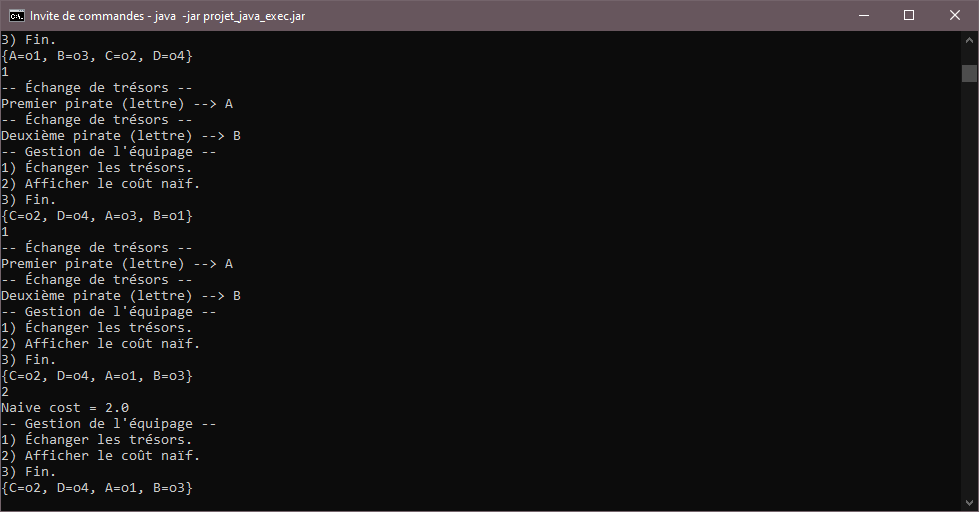
\includegraphics[width=16cm]{naive_cost}
\centering
\caption{Naive cost = 2.0}
\end{figure}
\section{Documentation et GitHub}
\paragraph{} Pour ce projet, et afin de faciliter le développement entre nous, nous avons décider d'utiliser la plateforme GitHub.
Elle nous a permis entre autres de partager notre code source et aussi d'héberger notre documentation en ligne. (en libre accès grâce à ReadTheDocs)
\subsection{Récupérer notre projet sur GitHub}
\paragraph{} Voici une commande pré-faite permettant de cloner notre dépôt git :
\begin{lstlisting}[style=BashStyle]
git clone https://github.com/Osmane-EL-MONTASER/projet-java-L3
\end{lstlisting}
\paragraph{} Le dépôt est public, ce qui vous permet de le cloner comme vous voulez et aussi de voir les différentes versions de notre programme.
Effectivement nous avions d'abord commencé une 1.0 sans implémenter les graphes, puis nous avons codé le même programme avec notre classe générique pour les graphes dans la 2.0.
\subsection{Récupérer notre documentation}
\paragraph{} Pour accéder à notre documentation Javadoc, veuillez vous rendre sur ce lien :
\end{document}